\section{Formule d'Euler}

On donne une formule d'Euler :
\[
  \frac{\pi^2}{9} = \frac{5^2}{(5^2-1)}\frac{7^2}{(7^2-1)}\frac{11^2}{(11^2-1)}\frac{13^2}{(13^2-1)}\frac{17^2}{(17^2-1)}\frac{19^2}{(19^2-1)}\dots
\]
En continuant ainsi avec la liste des nombres premiers à partir de 5.

\begin{enumerate}[(a)]
  \item \q{A quel nombre premier $k$ faut-il s'arrêter dans cette formule pour avoir $\frac{\pi^2}{9}$ à $10^{-4}$ près ?}

        \bigskip

        \begin{dinglist}{111}
          \item J'espère qu'il faut $k \leq 1 229$. Ainsi je peux utiliser la liste précédente, et boucler en faisant
          augmenter $k$ à chaque fois.

          Je créer donc une première fonction qui ressemble beaucoup à \il{prime} qui renvoie la liste des nombres
          premiers inférieurs à \il{n} :

          \codeFromFile{section-04/qa-1.py}


          \item Ensuite je crée la fonction qui renvoie le terme général de la formule d'Euler ci-dessus :

          \codeFromFile{section-04/qa-2.py}


          \item Enfin je calcule chaque terme du produit en allant un rang plus loin à chaque fois, puis je compare
          les rangs $k$ et $k-1$. Si la différence est inférieure à $10^{-4}$, on est bon :

          \codeFromFile{section-04/qa-3.py}

          \textit{\ul{Remarque} : je renvoie $k-1$ et non $k$ car pour $k=32$, on est à $10^{-5}$ et avec k=31 on est
            tout juste au dessus de $10^{-4}$}

          \item J'exécute \il{print(picarre(4))}
          Avec k = 31, on trouve une précision
          \il{eps = 0.00010185214032998324} soit une précision à $10^{-4}$ près. D'où :
          \begin{result}
            $k = 31$
          \end{result}

        \end{dinglist}
  \item \q{Idem pour avoir $\frac{\pi^2}{9}$ à $10^{-5}$ près ?}

        \bigskip

        J'exécute \il{print(picarre(5))} et trouve, pour $k = 79$, une précision
        \il{eps = 1.0226025770831981e-05} soit une précision à $10^{-5}$ près. Donc :
        \begin{result}
          Pour avoir $\frac{\pi^2}{9}$ à $10^{-5}$ près, il faut $k = 79$.
        \end{result}

  \item \q{En prenant 13 valeurs différentes d'erreurs égales à $\frac{1}{M}$ où $M$ est équirépartie entre $50$ et
          $10^{5}$, vérifier que dans la formule d'Euler, l'erreur est de l'ordre de $\frac{1}{kln(k)}$ où $k$ est le
          dernier nombre premier utilisé dans le produit.}

        \bigskip

        \begin{dinglist}{111}
          \item On commence par importer les librairies, et aussi par calculer la liste des 1 229 premiers nombres
          premiers, ça sera fait :

          \bigskip

          \codeFromFile{section-04/qc-1.py}

          \bigskip

          \item Bien-sûr, il faut un peu modifier la fonction \il{picarre} précédente :

          \bigskip

          \codeFromFile{section-04/qc-2.py}

          \item Enfin, on code ce qui est demandé :
          \codeFromFile{section-04/qc-3.py}

          \item
          Et on obtient ça :
          \begin{center}
            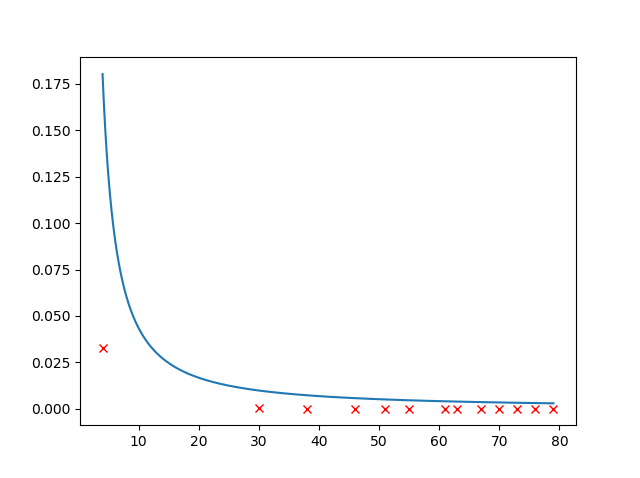
\includegraphics[scale=0.8]{section-04/qc-4.png}
          \end{center}
          Mais ce n'est pas très concluant... J'ai essayé de retourner $k$ et non $k-1$ dans la fonction \il{picarre},
          mais ça ne change pas grand chose\dots

        \end{dinglist}
\end{enumerate}
